\chapter{Body Plans and Common Ancestry}\label{ch:g10:common-ancestry}

Hold your arm out and count: one bone from shoulder to elbow, two from
elbow to wrist, a cluster of small bones in the wrist, five fingers. Now
look at the skeleton of a bat's wing, a whale's flipper, a horse's
foreleg, a frog's arm: the same one bone, two bones, cluster, and
digits, stretched, fused or shortened but never rearranged. Nobody
designing a wing from scratch would start from an arm. The resemblance
is the mark of something inherited, and this chapter is about reading
such marks --- in skeletons, in embryos, in molecules --- to reconstruct
the kinship of living things.

\section{The vertebrate body plan}

\begin{definition}[Body plan]\label{def:g10:common-ancestry:bodyplan}
The \emph{body plan}\index{body plan} of a group of organisms is the
common arrangement of their parts: the axes of symmetry and the
relative positions of the main organs, independently of size, shape
or way of life. The \emph{vertebrates}\index{vertebrate} --- fish,
amphibians, reptiles, birds, mammals --- share one plan: a body
symmetric about a vertical plane, with a front end carrying the head
and a back end; an internal skeleton whose axis is a column of
vertebrae protecting a dorsal nerve cord; the digestive tube running
ventrally, mouth in front, and the heart beneath it.
\end{definition}

\begin{omfigure}
\begin{tikzpicture}[font=\small, >=Stealth]
  % generic vertebrate side view
  \draw[thick, fill=omDef!6, rounded corners=14pt] (0,0) rectangle (9,3.2);
  \draw[thick, omThm] (0.6,2.5) -- (8.6,2.5);                      % nerve cord
  \foreach \x in {1.2,1.8,...,8.4} \draw[thick] (\x,2.15) -- (\x,2.35); % vertebrae
  \draw[thick] (1.0,2.25) -- (8.6,2.25);
  \draw[thick, omProp, fill=omProp!20] (0.5,1.4) .. controls (2,0.7) and (6,0.7) .. (8.6,1.2)
    .. controls (6,1.5) and (2,1.9) .. (0.5,1.4);                      % gut
  \draw[thick, omThm, fill=omThm!30] (2.3,0.75) circle (0.32);         % heart
  \node[anchor=west] at (9.4,2.5) {nerve cord (dorsal)};
  \draw[->] (9.35,2.5) -- (8.65,2.5);
  \node[anchor=west] at (9.4,2.0) {vertebral column};
  \draw[->] (9.35,2.0) -- (8.6,2.22);
  \node[anchor=west] at (9.4,1.2) {digestive tube (ventral)};
  \draw[->] (9.35,1.2) -- (8.65,1.2);
  \node[anchor=north] at (2.3,-0.1) {heart, beneath the tube};
  \draw[->] (2.3,-0.05) -- (2.3,0.4);
  \node[anchor=east] at (-0.1,1.4) {mouth};
  \draw[->] (-0.05,1.4) -- (0.45,1.4);
  \node[anchor=south, font=\small\itshape] at (4.5,3.3) {dorsal side};
  \node[anchor=north, font=\small\itshape] at (6.5,-0.05) {ventral side};
  \draw[<->, gray] (0,3.7) -- (9,3.7) node[midway, above, font=\scriptsize] {front--back axis};
\end{tikzpicture}

{\small The \omterm{def:g10:common-ancestry:bodyplan}{vertebrate} \omterm{def:g10:common-ancestry:bodyplan}{body plan}, in side view. Whatever the species,
the nerve cord runs along the back above the vertebral column, the
digestive tube along the belly, the heart beneath it near the front.
Insects and earthworms have the nerve cord on the ventral side: a
different plan.}
\end{omfigure}

\begin{example}[Same plan, different animals]\label{ex:g10:common-ancestry:sameplan}
A trout, a frog, a lizard, a pigeon and a mouse dissected side by side
show the plan in every case: the spinal cord in the back, protected by
vertebrae; the gut below it with a liver beside the stomach; the heart
in front, under the gut; paired limbs (or fins) attached to girdles of
bone. The differences --- gills or lungs, fins or legs, scales, feathers
or fur --- are all variations built on the same arrangement.
\end{example}

\section{Homologous organs}

\begin{definition}[Homology]\label{def:g10:common-ancestry:homology}
Two organs of two species are \emph{homologous}\index{homology} when
they have the same structure and the same position in the \omterm{def:g10:common-ancestry:bodyplan}{body plan}
--- built of the same parts in the same relations --- whatever their
present function. The forelimbs of tetrapods are the standard example:
one bone (humerus), two bones (radius and ulna), a cluster of wrist
bones, then the digits. Organs that perform the same function with a
different structure --- the wing of a bird and the wing of a fly --- are
merely \emph{analogous}, and say nothing about kinship.
\end{definition}

\begin{omfigure}
\begin{tikzpicture}[font=\small, line cap=round]
  % three stylised forelimbs: humerus (red), radius+ulna (blue), carpals (gray), digits (green)
  \tikzset{hum/.style={line width=6pt, omThm!70},
           ru/.style={line width=4pt, omDef!70},
           carp/.style={fill=gray!50, draw=gray!70},
           dig/.style={line width=3pt, omMeth!80}}
  % human arm
  \begin{scope}
    \draw[hum] (0,3.2) -- (0.2,1.9);
    \draw[ru] (0.1,1.85) -- (0.3,0.9); \draw[ru] (0.35,1.85) -- (0.5,0.9);
    \fill[carp] (0.15,0.7) rectangle (0.65,0.85);
    \foreach \dx in {-0.3,-0.12,0.05,0.22,0.4} \draw[dig] (0.4,0.7) -- ({0.4+\dx},-0.1);
    \node[anchor=north] at (0.4,-1.4) {human arm};
  \end{scope}
  % bat wing
  \begin{scope}[xshift=3.6cm]
    \draw[hum] (0,3.2) -- (0.4,2.3);
    \draw[ru] (0.4,2.3) -- (1.0,1.3);
    \fill[carp] (0.95,1.2) rectangle (1.25,1.35);
    \draw[dig] (1.1,1.2) -- (0.8,0.9);
    \foreach \a in {-0.6,-0.3,0.1,0.5} \draw[dig] (1.1,1.2) -- ({1.1+2.2*cos(-60+40*\a)},{1.2+2.2*sin(-60+40*\a)});
    \node[anchor=north] at (1.2,-1.4) {bat wing};
  \end{scope}
  % whale flipper
  \begin{scope}[xshift=8.0cm]
    \draw[hum] (0,3.2) -- (0.1,2.5);
    \draw[ru] (0.0,2.45) -- (0.05,1.9); \draw[ru] (0.3,2.45) -- (0.35,1.9);
    \fill[carp] (-0.05,1.6) rectangle (0.5,1.85);
    \foreach \dx in {-0.2,0.0,0.2,0.45} \draw[dig] ({0.22+0.5*\dx},1.6) -- ({0.22+\dx},0.2);
    \draw[gray!60, rounded corners=8pt] (-0.5,3.4) -- (-0.6,0.0) -- (0.9,-0.1) -- (0.9,3.4);
    \node[anchor=north] at (0.2,-1.4) {whale flipper};
  \end{scope}
  % legend
  \begin{scope}[xshift=10.4cm, yshift=2.2cm]
    \draw[hum] (0,1.0) -- (0.6,1.0); \node[anchor=west] at (0.7,1.0) {humerus};
    \draw[ru] (0,0.5) -- (0.6,0.5); \node[anchor=west] at (0.7,0.5) {radius, ulna};
    \fill[carp] (0.05,-0.08) rectangle (0.55,0.08); \node[anchor=west] at (0.7,0) {wrist bones};
    \draw[dig] (0,-0.5) -- (0.6,-0.5); \node[anchor=west] at (0.7,-0.5) {digits};
  \end{scope}
\end{tikzpicture}

{\small Three \omterm{def:g10:common-ancestry:homology}{homologous} forelimbs, schematically: the same bones in
the same order, lengthened into a wing, flattened into a flipper.
Function differs; structure and position do not.}
\end{omfigure}

\begin{omfigure}
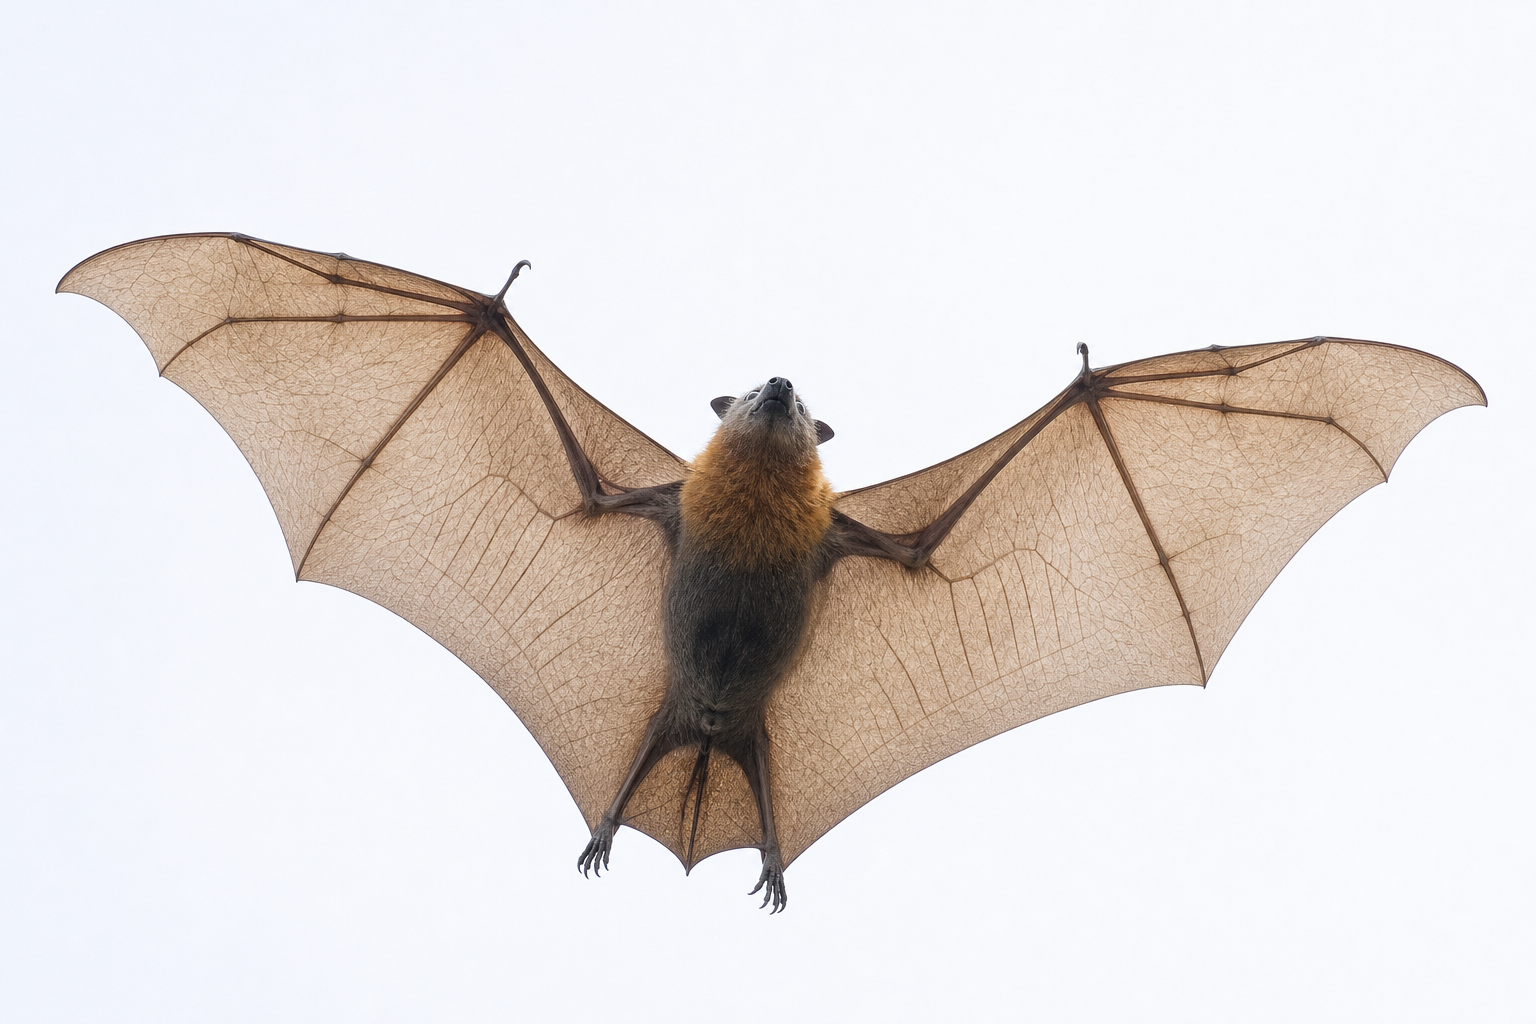
\includegraphics[width=0.6\linewidth]{images/book2/ai/g10-ancestry-bat-wing.png}

{\small A bat in flight: the wing membrane is stretched over
enormously lengthened finger bones. The hand of the mammalian plan,
turned into a wing.}
\end{omfigure}

\begin{proposition}[Homology reveals kinship]\label{prop:g10:common-ancestry:kinship}
Shared \omterm{def:g10:common-ancestry:homology}{homologous} structures are inherited from a common ancestor
that possessed them; the more such structures two species share, the
closer their kinship. The tetrapod limb is found in every land
\omterm{def:g10:common-ancestry:bodyplan}{vertebrate} because all descend from one ancestral lineage that had it;
a bat's wing is a modified arm because bats descend from mammals with
arms, not from birds.
\end{proposition}
\begin{proof}[Evidence]
Three independent lines converge. \emph{Fossils}: the sequence of dated
rocks contains forms with intermediate combinations of characters ---
fish with limb-like fins and a neck 375 million years ago, then
four-legged animals with fish-like tails; \emph{Archaeopteryx}, 150
million years old, with feathers and wings but also teeth, clawed
fingers and a long bony tail. \emph{Embryos}: all \omterm{def:g10:common-ancestry:bodyplan}{vertebrate} embryos
pass through a stage with gill pouches, a tail and a notochord ---
structures kept in the adult fish, reworked or lost in the others.
\emph{Molecules}: as \cref{ch:g10:universal-dna} showed, all share
\omterm{def:g10:universal-dna:information}{DNA} and the same \omterm{def:g10:universal-dna:gene}{genes}, and the differences between the versions of
one \omterm{def:g10:universal-dna:gene}{gene} rank species exactly as the anatomy does.
\end{proof}

\begin{omfigure}
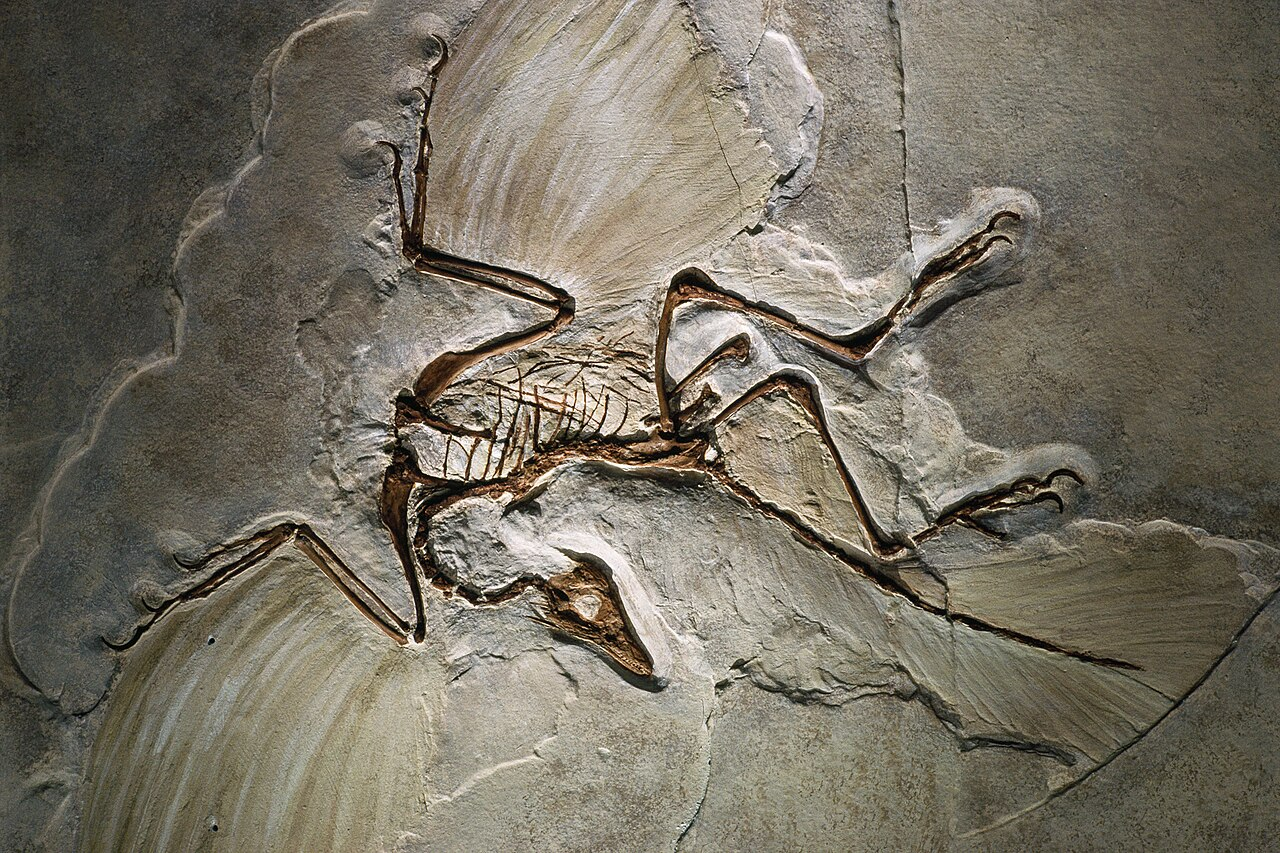
\includegraphics[width=0.5\linewidth]{images/book1/archaeopteryx.jpg}

{\small \emph{Archaeopteryx}, 150 million years old: feathered wings
and a wishbone like a bird, teeth, clawed fingers and a long bony
tail like a small dinosaur. A fossil combining the characters of two
groups is what common ancestry predicts. Photo James L.~Amos, CC0.}
\end{omfigure}

\section{Nested groups}

\begin{method}[Grouping by shared characters]\label{met:g10:common-ancestry:grouping}
Kinship groups are built by shared \emph{derived} characters ---
features that appeared once in an ancestor and were inherited by all
its descendants.
\begin{enumerate}
  \item List the species and a set of characters (vertebral column;
        four limbs; egg with a shell or its equivalent, the amniotic
        egg; feathers; hair and milk; and so on).
  \item For each character, note which species possess it.
  \item A character shared by a subset defines a group: all species
        with four limbs are the tetrapods; among them, all with an
        amniotic egg are the amniotes; among those, all with hair are
        the mammals.
  \item Draw the groups as nested boxes, or as a tree in which each
        node is the common ancestor in which the character appeared.
        A group must contain \emph{all} the descendants of that
        ancestor: "fish" or "reptiles" in the everyday sense are not
        such groups.
\end{enumerate}
\end{method}

\begin{omfigure}
\begin{tikzpicture}[font=\small]
  \node[draw, rounded corners, thick, fill=omDef!6, minimum width=12.2cm, minimum height=4.6cm] (v) at (0,0) {};
  \node[anchor=north west] at (v.north west) {\ \textbf{vertebrates}: vertebral column};
  \node[anchor=south west] at (v.south west) {\ trout};
  \node[draw, rounded corners, thick, fill=omMeth!8, minimum width=9.6cm, minimum height=3.5cm] (t) at (0.9,-0.25) {};
  \node[anchor=north west] at (t.north west) {\ \textbf{tetrapods}: four limbs};
  \node[anchor=south west] at (t.south west) {\ frog};
  \node[draw, rounded corners, thick, fill=omProp!10, minimum width=7.0cm, minimum height=2.4cm] (a) at (1.8,-0.5) {};
  \node[anchor=north west] at (a.north west) {\ \textbf{amniotes}: amniotic egg};
  \node[anchor=south west] at (a.south west) {\ lizard\quad pigeon};
  \node[draw, rounded corners, thick, fill=omThm!10, minimum width=3.7cm, minimum height=1.3cm] (m) at (3.2,-0.75) {};
  \node[anchor=north west] at (m.north west) {\ \textbf{mammals}: hair, milk};
  \node[anchor=south west] at (m.south west) {\ mouse\quad human};
\end{tikzpicture}

{\small Nested kinship groups of five \omterm{def:g10:common-ancestry:bodyplan}{vertebrates}. Each box is defined
by a character that appeared once, in the common ancestor of everything
inside it. The pigeon is inside "amniotes" with the lizard: the
lizard is closer kin to the pigeon than to the frog.}
\end{omfigure}

\begin{example}[Reading the boxes]\label{ex:g10:common-ancestry:reading}
Which is the mouse's closest relative among trout, frog, lizard and
pigeon? The smallest box containing the mouse and another species is
"amniotes", which holds the lizard and the pigeon: they are equally
close, both nearer to the mouse than the frog is, and the frog nearer
than the trout. That a lizard is closer to a pigeon than to a frog
surprises most people; the shelled egg, a character no frog has,
settles it.
\end{example}

\section{Kinship in the molecules}

\begin{proposition}[Molecular kinship]\label{prop:g10:common-ancestry:molecular}
Since all living things descend from common ancestors, a \omterm{def:g10:universal-dna:gene}{gene} present
in two species is a modified copy of the ancestral \omterm{def:g10:universal-dna:gene}{gene}, and the
number of differences between the two copies grows with the time since
the species separated. Comparing the sequence of one \omterm{def:g10:universal-dna:gene}{gene}, or of the
\omterm{def:g10:chemistry-of-life:families}{protein} it codes for, across species therefore measures kinship, and
the resulting groupings agree with those drawn from anatomy.
\end{proposition}
\admitted

\begin{example}[Cytochrome c]\label{ex:g10:common-ancestry:cytochrome}
Cytochrome c is a \omterm{def:g10:chemistry-of-life:families}{protein} of about 104 \omterm{def:g10:chemistry-of-life:families}{amino acids} used in
respiration by every eukaryote. Compared with the human sequence, the
chimpanzee's differs at 0 positions, the mouse's at 9, the chicken's
at 13, the frog's at 18, the tuna's at 21, and yeast's at 45. Ranked
by differences, the species fall into exactly the boxes of the
previous figure: mammal, then amniote, then tetrapod, then \omterm{def:g10:common-ancestry:bodyplan}{vertebrate},
then eukaryote.
\end{example}

\begin{remark}[Unity and kinship]\label{rem:g10:common-ancestry:unity}
The unity of composition (\cref{ch:g10:chemistry-of-life}), of the \omterm{def:g10:cells-common-unit:cell}{cell}
(\cref{ch:g10:cells-common-unit}), of the genetic molecule
(\cref{ch:g10:universal-dna}) and now of \omterm{def:g10:common-ancestry:bodyplan}{body plans} and \omterm{def:g10:universal-dna:gene}{gene} sequences
is one fact seen four times: living things resemble each other because
they are related, and they are related because they descend from
common ancestors. The diversity of \cref{ch:g10:biodiversity-scales}
is the outcome of that descent with modification, over the time the
fossil record measures. How the modifications arise and spread is the
subject of the final year.
\end{remark}

\section{Exercises}

\begin{exercise}[$\star$]\label{exo:g10:common-ancestry:1}
List four features of the \omterm{def:g10:common-ancestry:bodyplan}{vertebrate} \omterm{def:g10:common-ancestry:bodyplan}{body plan}.
\end{exercise}

\begin{exercise}[$\star$]\label{exo:g10:common-ancestry:2}
Define \omterm{def:g10:common-ancestry:homology}{homologous} organs and give the standard example.
\end{exercise}

\begin{exercise}[$\star$]\label{exo:g10:common-ancestry:3}
Are the wing of a bird and the wing of a butterfly \omterm{def:g10:common-ancestry:homology}{homologous} or
analogous? Justify.
\end{exercise}

\begin{exercise}[$\star$]\label{exo:g10:common-ancestry:4}
Using the nested-boxes figure, say which is closer to the frog: the
trout or the lizard.
\end{exercise}

\begin{exercise}[$\star$]\label{exo:g10:common-ancestry:5}
Which three lines of evidence support the idea that shared homologies
come from a common ancestor?
\end{exercise}

\begin{exercise}[$\star\star$]\label{exo:g10:common-ancestry:6}
A whale has a flipper with the tetrapod bone pattern, breathes air,
suckles its young, and has tiny hip bones unattached to any leg. Which
box of the figure does it belong to? What do the hip bones suggest?
\end{exercise}

\begin{exercise}[$\star\star$]\label{exo:g10:common-ancestry:7}
Add the crocodile (four limbs, amniotic egg, scales, no hair) and the
salamander (four limbs, egg laid in water without shell) to the nested
boxes.
\end{exercise}

\begin{exercise}[$\star\star$]\label{exo:g10:common-ancestry:8}
Explain why "fish" (trout, shark, lungfish\dots) is not a kinship group
in the sense of \cref{met:g10:common-ancestry:grouping}, knowing that
the lungfish is closer to the frog than to the trout.
\end{exercise}

\begin{exercise}[$\star\star$]\label{exo:g10:common-ancestry:9}
Using the cytochrome c data, rank the human's relatives from closest
to most distant and check the ranking against the anatomical boxes.
\end{exercise}

\begin{exercise}[$\star\star$]\label{exo:g10:common-ancestry:10}
Human embryos of four weeks have gill pouches in the neck and a tail,
both of which disappear later. What does this observation contribute
to the argument of the chapter?
\end{exercise}

\begin{exercise}[$\star\star$]\label{exo:g10:common-ancestry:11}
\emph{Archaeopteryx} has feathers and a long bony tail. Explain why a
fossil with a mixture of characters is expected under common ancestry
and would be puzzling without it.
\end{exercise}

\begin{exercise}[$\star\star\star$]\label{exo:g10:common-ancestry:12}
The eyes of an octopus and of a human are both cameras with a lens and
a retina, yet they develop from different tissues and the octopus
retina is wired the other way round. \omterm{def:g10:common-ancestry:homology}{Homologous} or analogous? What
would each answer imply about their common ancestor?
\end{exercise}

\begin{exercise}[$\star\star\star$]\label{exo:g10:common-ancestry:13}
Cytochrome c differs between human and mouse at 9 positions, between
human and chicken at 13, and between mouse and chicken at 13 as well.
Explain why the last two numbers are expected to be equal (or nearly)
if differences accumulate steadily with time.
\end{exercise}

\begin{exercise}[$\star\star\star$]\label{exo:g10:common-ancestry:14}
Snakes have no limbs, yet they are placed among the tetrapods. On what
evidence, and what does "tetrapod" then mean?
\end{exercise}

\begin{exercise}[$\star\star\star$]\label{exo:g10:common-ancestry:15}
A friend argues that similar animals simply live in similar ways, and
that is why they look alike. Use the forelimb, the embryo and the
molecule to explain what that argument cannot account for.
\end{exercise}

\section{Problem: One Tree, Two Kinds of Evidence}

\begin{problem}[{Weekend problem --- five vertebrates, their skeletons
and one of their proteins: kinship built from anatomy, rebuilt from
molecules, and the two compared}]
\label{pb:g10:common-ancestry:1}
The class studies five species: a trout, a frog, a lizard, a pigeon and
a mouse. Character table (1 = present, 0 = absent):

\begin{center}
\begin{tabular}{lccccc}
 & trout & frog & lizard & pigeon & mouse \\ \hline
vertebral column & 1 & 1 & 1 & 1 & 1 \\
four limbs & 0 & 1 & 1 & 1 & 1 \\
amniotic egg & 0 & 0 & 1 & 1 & 1 \\
feathers & 0 & 0 & 0 & 1 & 0 \\
hair and milk & 0 & 0 & 0 & 0 & 1 \\
\end{tabular}
\end{center}

Number of differences in cytochrome c (rounded):

\begin{center}
\begin{tabular}{lcccc}
 & frog & lizard & pigeon & mouse \\ \hline
trout & 19 & 20 & 21 & 21 \\
frog & & 16 & 17 & 18 \\
lizard & & & 12 & 14 \\
pigeon & & & & 13 \\
\end{tabular}
\end{center}

\medskip
\noindent\textbf{Part I --- The skeletons.}
\begin{enumerate}
  \item Which character is shared by all five? Which group does it
        define?
  \item Which characters define a group of four, a group of three?
        Name the groups.
  \item Feathers and hair are each found in one species. Can such a
        character define a kinship group among these five? What is it
        useful for?
  \item Draw the nested boxes for the five species, or the
        corresponding tree.
  \item The frog's forelimb has the humerus, radius--ulna, wrist and
        digit pattern; the trout's pectoral fin has rays of bone
        fanning from a small base. Which is \omterm{def:g10:common-ancestry:homology}{homologous} to your arm?
        Which character of the table does this correspond to?
\end{enumerate}

\medskip
\noindent\textbf{Part II --- The molecule.}
\begin{enumerate}[resume]
  \item From the second table, which two species are the closest
        pair? Which species is most distant from all the others?
  \item Rank the mouse's relatives from closest to most distant using
        the molecule alone.
  \item Do the same for the frog. Is the ranking consistent with the
        boxes of Part I?
  \item The lizard--pigeon distance (12) is smaller than the
        lizard--mouse distance (14). What does this suggest about the
        branching order within the amniotes, and does the character
        table say anything about it?
  \item Explain why the trout's distances to the four others are all
        about equal (19--21).
\end{enumerate}

\medskip
\noindent\textbf{Part III --- Comparing the two.}
\begin{enumerate}[resume]
  \item List the groupings both kinds of evidence agree on.
  \item Why is agreement between an anatomical and a molecular
        ranking strong evidence, when either alone could be
        questioned?
  \item Suppose a sixth species, a bat, were added: forelimb with the
        tetrapod pattern, amniotic egg, hair and milk, cytochrome c
        differing from the mouse at 8 positions and from the pigeon
        at 13. Where does it go? Why does its wing not put it with the
        pigeon?
  \item The cytochrome c of a chimpanzee is identical to the human
        one, yet the two species differ visibly. What does this say
        about which \omterm{def:g10:universal-dna:gene}{genes} cytochrome c comparisons can and cannot
        inform us about?
  \item A yeast's cytochrome c differs from all five at about 45
        positions. What box, larger than "\omterm{def:g10:common-ancestry:bodyplan}{vertebrates}", does the
        yeast share with them?
\end{enumerate}

\medskip
\noindent\textbf{Part IV --- Time and the tree.}
The fossil record dates the separation of the mouse and pigeon
lineages to about 320 million years ago.
\begin{enumerate}[resume]
  \item If differences accumulate steadily in both lineages, how many
        differences appear per 100 million years along one lineage?
        (Use the mouse--pigeon distance, remembering that both
        lineages have been changing.)
  \item Use that rate to estimate the age of the separation of the
        frog lineage from the amniotes, from the frog--mouse and
        frog--pigeon distances.
  \item Estimate likewise the separation of the trout lineage.
  \item Fossils place the first tetrapods at about 370 million years
        ago and the first \omterm{def:g10:common-ancestry:bodyplan}{vertebrates} with jaws well over 420. Compare
        with your estimates and comment on the agreement.
  \item State the result in one sentence: what the two kinds of
        evidence, taken together, establish about the five species,
        and what the molecule adds that the skeleton cannot.
\end{enumerate}
\end{problem}
